\documentclass[11pt]{article}
\usepackage{fullpage}
\usepackage{epic}
\usepackage{eepic}
\usepackage{graphicx}
\usepackage{algorithm,algorithmic}
 \usepackage{enumitem}


\usepackage{amsfonts,mathrsfs,amsmath}
\usepackage{hyperref}
\usepackage{color}
\usepackage{geometry}
\usepackage{changepage}
\pagestyle{empty}
\setlength{\oddsidemargin}{0in}
\setlength{\topmargin}{0in}
\setlength{\textwidth}{6.8in}
\setlength{\textheight}{9.5in}
\usepackage {tikz}
\usetikzlibrary{shapes,arrows, positioning}
\usepackage{caption}


\begin{document}

\setlength{\fboxrule}{.5mm}\setlength{\fboxsep}{1.2mm}
\newlength{\boxlength}\setlength{\boxlength}{\textwidth}
\addtolength{\boxlength}{-4mm}
\begin{center}\framebox{\parbox{\boxlength}{\bf
Robot Learning \hfill Assignment 1\\
CS 4756 Spring 2024 \hfill Due 11:59pm Sunday,  February 18}}\end{center}
\vspace{5mm}

\def\ind{\hspace*{0.3in}}
\def\gap{0.2in}


\vskip \gap \noindent{\bf (1) Exploring Markov Decision Processes (5 points)} 

\begin{figure}[h!]
\centering
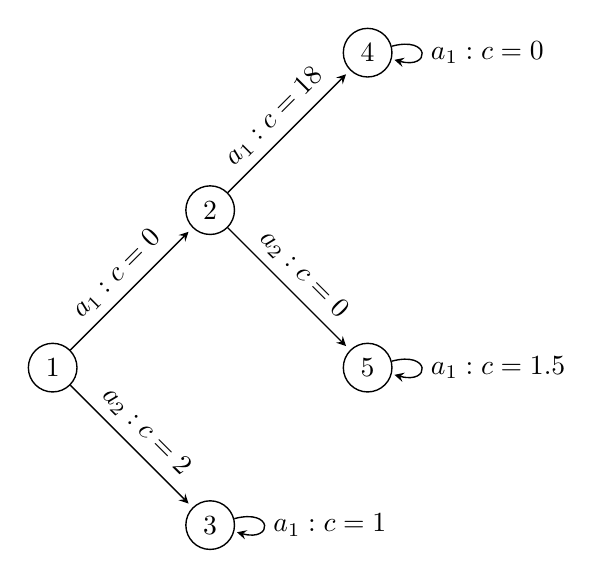
\begin{tikzpicture}[->,>=stealth, shorten >=2pt, line width = 0.5 pt,
node distance = 2 cm]

\node [circle, draw] (one) {1};
\node [circle, draw] (two) [right of=one, above of=one] {2};
\path (one) edge node [above,sloped] {$a_1 : c = 0$} (two);
\node [circle, draw] (three) [right of=one, below of=one] {3};
\path (one) edge node [above,sloped] {$a_2 : c = 2$} (three);
\path (three) edge  [loop right] node  {$a_1 : c = 1$}(three);


\node [circle, draw] (four) [right of=two, above of=two] {4};
\path (two) edge node [above,sloped] {$a_1 : c = 18$}(four);
\path (four) edge [loop right] node  {$a_1 : c = 0$}(four);
\node [circle, draw] (five) [right of=two, below of=two] {5};
\path (two) edge node [above,sloped] {$a_2 : c = 0$} (five);
\path (five) edge [loop right] node  {$a_1 : c = 1.5$}(five);

\end{tikzpicture}
\caption{\label{fig:prob1} MDP for Problem 1}
\end{figure}

\noindent Compute the optimal value function $V^{*}$ and the corresponding optimal policy $\pi^{*}$ for each state in Fig.~\ref{fig:prob1} for a discount factor of $\gamma = 0.9$ in the infinite horizon setting. 

\vspace{1em}
Notes:
\begin{itemize}
    \item Initial State is always State 1. 
    \item Each edge of the MDP is labeled in the following format: "\{action\} : \{cost of action to complete transition\}". Thus, the problem formulation involves a minimization of cost, rather than a maximization of a reward as may be seen elsewhere.
    \item Action $a_1$ at states 3, 4, and 5 must be taken infinitely if those states are ever reached.
\end{itemize}


\newpage

\noindent{\bf (2) A Story of Three Cliffs: Behavior Cloning and DAgger (10 points)}
\vskip 0.1in

\noindent In this question, we are going to be thinking about robots falling off of cliffs and trying to get back on. We will look at three types of cliffs with varying levels of difficulty, and compare how well behavior cloning (BC) performs with respect to DAgger. 

\noindent In all of the following parts, we will consider an infinite horizon setting with a discount factor of $\gamma$. Each part considers a Cliff MDP, where there exists a path atop the cliff consisting of ``safe'' states as well as a path to fall off the cliff from any point and land at the bottom, which we denote at $s_x$. 

For each variant of the MDP, compute the tightest possible upper bounds (in terms of big-O) for the following quantities:
\begin{itemize}
    \item $J(\pi_{BC})$: Expected total discounted sum of costs for Behavior Cloning
    \item $J(\pi_{DAgger})$: Expected total discounted sum of costs for DAgger
\end{itemize}
Important notes and assumptions:
\begin{itemize}
    \item An agent begins at state $s_0$
    \item The expert will always follow an optimal trajectory, thus the expert policy will incur 0 cost
    \item At each state the learner (both BC and DAgger) visits that the expert has also visited (i.e. all the safe states), it will make a mistake with probability $\epsilon$ and fall off the cliff
    \item Once the the BC learner has reached an unknown state, in the worst case with probability 1 it will continue to make mistakes and stay at the bottom of the cliff
    \item In contrast, the DAgger learner will query the expert to determine its next action, being able to complete a recovery action with probability 1 (if it exists)
    \item Assume that $0 < \epsilon \ll 1$, and $0 < 1 - \gamma \ll 1$ to simplify your calculations.
\end{itemize}

\noindent{\bf (a) Cliff-Easy} 
\begin{figure}[h!]
\centering
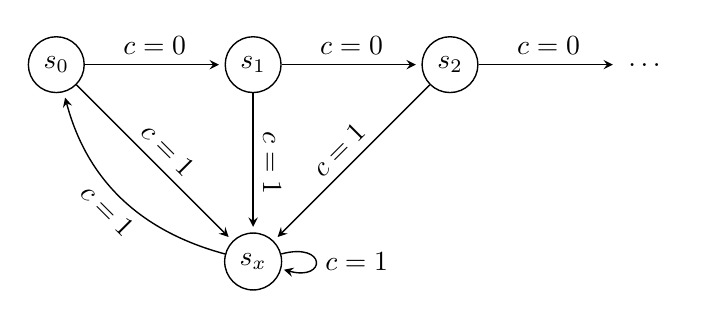
\begin{tikzpicture}[->,>=stealth, shorten >=2pt, line width = 0.5 pt,
node distance = 2.5 cm]

\node [circle, draw] (zero) {$s_0$};
\node [circle, draw] (one) [right of=zero] {$s_1$};
\path (zero) edge node [above] {$c = 0$} (one);
\node [circle, draw] (two) [right of=one] {$s_2$};
\path (one) edge node [above] {$c = 0$} (two);
\node (three) [right of=two] {\ldots};
\path (two) edge node [above] {$c = 0$} (three);

\node [circle, draw] (cliff) [below of=one] {$s_x$};
\path (zero) edge node [above,sloped] {$c = 1$} (cliff);
\path (one) edge node [above,sloped] {$c = 1$} (cliff);
\path (two) edge node [above,sloped] {$c = 1$} (cliff);

\path (cliff) edge [bend left] node [below,sloped] {$c = 1$} (zero); 
\path (cliff) edge [loop right] node  {$c = 1$}(cliff);


\end{tikzpicture}
\end{figure}

\noindent Cliff-Easy: The safe states $s_i$ can either transition to $s_{i+1}$ with $c = 0$ or $s_x$ with $c = 1$, but there exists a recovery action from $s_x$ to return to $s_0$ with $c = 1$. Bounds should be in terms of $\epsilon, \gamma$.


\vskip 0.1in
\noindent{\bf (b) Cliff-Medium}
\begin{figure}[h!]
\centering
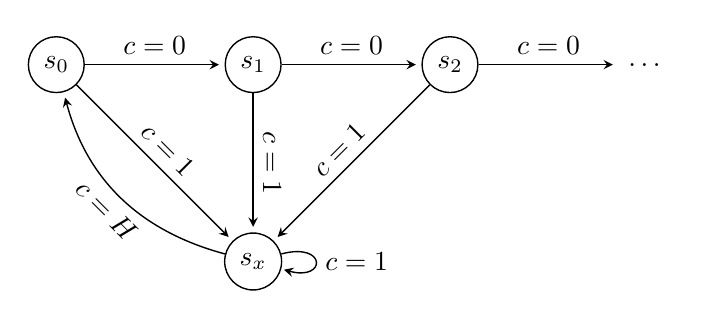
\begin{tikzpicture}[->,>=stealth, shorten >=2pt, line width = 0.5 pt,
node distance = 2.5 cm]

\node [circle, draw] (zero) {$s_0$};
\node [circle, draw] (one) [right of=zero] {$s_1$};
\path (zero) edge node [above] {$c = 0$} (one);
\node [circle, draw] (two) [right of=one] {$s_2$};
\path (one) edge node [above] {$c = 0$} (two);
\node (three) [right of=two] {\ldots};
\path (two) edge node [above] {$c = 0$} (three);

\node [circle, draw] (cliff) [below of=one] {$s_x$};
\path (zero) edge node [above,sloped] {$c = 1$} (cliff);
\path (one) edge node [above,sloped] {$c = 1$} (cliff);
\path (two) edge node [above,sloped] {$c = 1$} (cliff);

\path (cliff) edge [bend left] node [below,sloped] {$c = H$} (zero); 
\path (cliff) edge [loop right] node  {$c = 1$}(cliff);


\end{tikzpicture}
\end{figure}

\noindent Cliff-Medium: The safe states $s_i$ can either transition to $s_{i+1}$ with $c = 0$ or $s_x$ with $c = 1$, but there exists a recovery action from $s_x$ to return to $s_0$ with $c = H$. Bounds should be in terms of $\epsilon, \gamma, H$.


\vskip 1.2in
\noindent{\bf (c) Cliff-Hard}
\begin{figure}[h!]
\centering
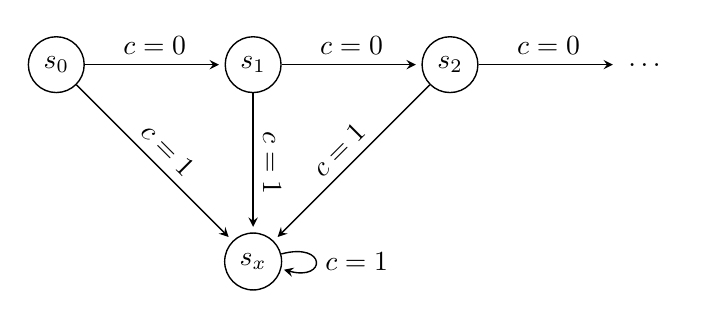
\begin{tikzpicture}[->,>=stealth, shorten >=2pt, line width = 0.5 pt,
node distance = 2.5 cm]

\node [circle, draw] (zero) {$s_0$};
\node [circle, draw] (one) [right of=zero] {$s_1$};
\path (zero) edge node [above] {$c = 0$} (one);
\node [circle, draw] (two) [right of=one] {$s_2$};
\path (one) edge node [above] {$c = 0$} (two);
\node (three) [right of=two] {\ldots};
\path (two) edge node [above] {$c = 0$} (three);

\node [circle, draw] (cliff) [below of=one] {$s_x$};
\path (zero) edge node [above,sloped] {$c = 1$} (cliff);
\path (one) edge node [above,sloped] {$c = 1$} (cliff);
\path (two) edge node [above,sloped] {$c = 1$} (cliff);

\path (cliff) edge [loop right] node  {$c = 1$}(cliff);
\end{tikzpicture}
\end{figure}

\noindent Cliff-Hard: The safe states $s_i$ can either transition to $s_{i+1}$ with $c = 0$ or $s_x$ with $c = 1$, but there is NO recovery action at $s_x$. Bounds should be in terms of $\epsilon, \gamma$.


Finally, comment on the following: How does the gap between DAgger and BC change as we vary the $H$ in cliff-medium from $1$ to $\frac{1}{1-\gamma}$? What is the explanation for this trend?
\newpage


\noindent{\bf (3) [Extra Credit] Pitfalls of DAgger (5 points)}  

\noindent In this problem, we explore the performance bound of a policy learned by DAgger in an interesting MDP with multiple routes to a final goal state.

\begin{figure}[h!]
\centering
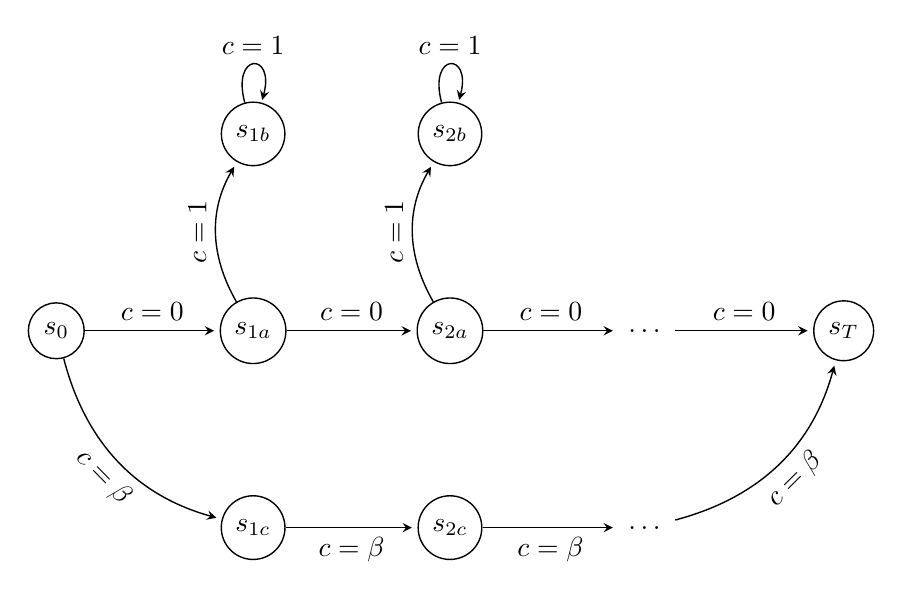
\begin{tikzpicture}[->,>=stealth, shorten >=2pt, line width = 0.5 pt,
node distance = 2.5 cm]

\node [circle, draw] (zero) {$s_0$};
\node [circle, draw] (one) [right of=zero] {$s_{1a}$};
\path (zero) edge node [above] {$c = 0$} (one);
\node [circle, draw] (two) [right of=one] {$s_{2a}$};
\path (one) edge node [above] {$c = 0$} (two);
\node (three) [right of=two] {\ldots};
\path (two) edge node [above] {$c = 0$} (three);
\node [circle, draw] (T) [right of=three] {$s_T$};
\path (three) edge node [above] {$c = 0$} (T);

\node [circle, draw] (alt1) [below of=one] {$s_{1c}$};
\node [circle, draw] (alt2) [below of=two] {$s_{2c}$};
\node (alt3) [right of=alt2] {\ldots};
\path (alt2) edge node [below] {$c = \beta$} (alt3);
\path (alt3) [bend right] edge node [below, sloped] {$c = \beta$} (T);

\node [circle, draw] (oneb) [above of=one] {$s_{1b}$};
\path (one) [bend left] edge node [above, sloped] {$c = 1$} (oneb);
\node [circle, draw] (twob) [above of=two] {$s_{2b}$};
\path (two) [bend left] edge node [above, sloped] {$c = 1$} (twob);
\path (oneb) edge [loop above] node  {$c = 1$}(oneb);
\path (twob) edge [loop above] node  {$c = 1$}(twob);

\path (zero) edge [bend right] node [below,sloped] {$c = \beta$} (alt1); 
\path (alt1) edge [right] node [below] {$c = \beta$} (alt2); 

\end{tikzpicture}
\caption*{Two ways to the goal}
\end{figure}

\noindent The MDP has two routes from the start $s_0$ to the goal $s_T$: 
\begin{enumerate}
    \item One route is the optimal route with action cost $0$ that the expert takes. There is, however, a caveat. The route passes over a bridge ($s_{1a}, s_{2a}, \dots,$) where a mistake can result in falling off the path into a ditch ($s_{1b}, s_{2b}, \dots)$. Once in the ditch, there is no recovery.
    \item One route is a long detour with action cost $\beta$. 
\end{enumerate}

\noindent Assume the following about our learner
\begin{itemize}
\item On states on the bridge, ($s_{1a}, s_{2a}, \dots,$), the learner makes a mistake with probability $\epsilon$. 
\item On all other states, it can perfectly imitate the expert. 
\end{itemize}

\noindent Compute the upper bound on $J(\pi_{DAgger})$, the expected total cost of trajectories for a DAgger policy over $T$ timesteps. Now, compute the cost of the best policy in the learner's class, $J(\pi^\star_{L})$. 
\begin{itemize}
\item  What is surprising about DAgger's performance specifically from this MDP based on this bound? Does DAgger find the best policy in the learner's policy class? 
\item In a few sentences, can you describe a real-world example that has a similar characteristic as this MDP? 
\end{itemize}
\end{document}



